
% Due Date: 6/30/14

\chapter{Physical Dependence Analysis}
\label{chapter:physical}

After tasks have completed the logical dependence
analysis stage of the Legion task pipeline, they
then proceed to the mapping stage of the pipeline
(see Chapter~\ref{chapter:arch}). The process
of mapping entails selecting a processor on which
to execute each task and then determining memories
in which to place physical instances for each
of the logical regions on which the task has requested
privileges. It is the responsibility of the runtime
to compute all of the data movement operations and
preconditions necessary for actually executing a
task in accordance with the requested logical 
region privileges and coherence. We refer to this
process as physical dependence analysis as it 
involves actually computing the operations necessary
for mapping a Legion application onto real hardware.

To ensure that dependences and data movement 
operations are determined correctly, a task $T$ 
is only allowed to map when all of the other tasks 
in the dynamic dependence graph on which $T$
has a dependence have mapped. This invariant
guarantees that when a task $T$ maps, it
will see the correct version of the meta-data
stored in the physical state of the region
tree forest and pick up any necessary dependences
on other tasks and operations that came before
$T$ in program order. An important property of
this invariant is that it permits Legion to 
map some tasks while logical dependence
analysis is being performed on other tasks. It
is impossible for task $T$ to record a mapping
dependence on any task that comes after it in
program order. This property allows Legion to
execute these stages of the pipeline in parallel 
for different tasks, aiding in the
latency hiding of the dynamic analysis.

In many ways the physical dependence analysis
for the mapping stage is similar to the logical 
dependence analysis: both algorithms involve 
traversals over the region tree forest to determine
dependences. However, there are two primary differences. 
First, tasks can begin physical dependence
analysis once all their mapping dependences
have been satisfied, permitting multiple tasks to 
be performing their physical dependence analysis
in parallel. Second, the state maintained in
the region tree forest will be different: the
runtime must track the various physical instances
of logical regions as well as the low-level events 
necessary for computing preconditions for low-level
runtime operations.

In this chapter we describe the physical 
dependence analysis that implements the
mapping stage of the task pipeline.  We begin
in Section~\ref{sec:phytraversal} by giving
a general overview of the traversal algorithm.
In Section~\ref{sec:phystree} we cover
the details of the data structures and 
optimizations we apply to make the physical
region tree traversal fast. 
Section~\ref{sec:physicalcases} covers
the implementation of several important
features of the Legion programming model
including virtual mappings, reduction
instances, composite instances, and compound 
region requirements. Finally, in 
Section~\ref{sec:paratraversal} we describe 
the necessary algorithms for enabling 
parallel traversal of the region
tree forest for non-interfering tasks.

\section{Physical Region Tree Traversal Algorithm}
\label{sec:phytraversal}
The physical region tree traversal algorithm is
in some ways similar to the logical region tree
traversal algorithm described in 
Chapter~\ref{chapter:logical}.  However, the 
goal of the physical traversal algorithm is not
to construct a dynamic dependence graph, but instead
to issue the appropriate operations to the 
Legion low-level runtime (see 
Section~\ref{subsec:lowlevel}) necessary for the
execution of tasks and other operations. 
Since the issuing of low-level operations
also corresponds to the binding of an application
to the hardware, the physical traversal algorithm
makes several mapper queries to determine
how each task should be mapped onto the target
hardware, ensuring that all decisions that
impact performance can be controlled by the
application developer. A partial semantics of
these mapper calls are given in this chapter,
while a complete description of the queries that
can be made to mapper objects can be found in
Chapter~\ref{chapter:mapping}.

In order to map a task, a target processor must
be first be selected via a mapping query. After
the processor is selected the runtime requests
that a mapper determine a ranking of memories
for each region requirement by an additional
mapping call. Based on these rankings, the runtime
attempts to map each of the region requirements
to a physical instance in one of the memories
in the target ranking\footnote{As part of this
process, the runtime also filters memories that 
are not visible from the target processor to 
maintain the correctness of the eventual mapping.}.
In order to map each of the different region
requirements, the runtime either locates or 
tries to create a physical instance in one of
the target memories. After a physical instance
is selected, the necessary copy operations are
determined and event dependences computed. To
perform these actions for each region requirement
of a task, four different stages are required. Each 
stage requires a traversal of a different
component of the physical state of the region
tree forest. We discuss each of these different 
traversals in turn.

\subsection{Premapping Traversal}
\label{sec:premapping}
The first traversal of the region tree is
the {\em premapping traversal}. For each
region requirement in the task, the 
premapping traversal walks the physical
region tree from where the parent task had
privileges to where region requirement is
requesting privileges similar to logical
region traversal. However, instead of searching
for interfering tasks, this traversal 
{\em opens} all sub-trees along the path and
performs any necessary close operations 
recorded by the logical traversal in 
Section~\ref{subsec:logicalstate} that have
yet to be performed. The intuition is that
the logical dependence analysis algorithm ensures
that tasks map in the proper order by 
recording dependences, therefore, in order
to guarantee that the physical region tree
remains in the proper state, only the open
and close operations need to be performed
during this first stage. If any close 
operations along the path have already been
performed by another task in the same epoch
then they can be skipped.

Unlike close operations in the logical region
tree traversal that only mutate the state
of the meta-data in the region tree forest,
close operations performed on the physical
state are translated to low-level runtime
operations.  To perform a close operation,
a physical instance of the logical region 
at the root of the sub-tree to be closed,
must first be either selected or created.
(Note this physical instance must also
have sufficient space for all the fields
that are being closed.) Since the decisions
about placement and layout of this physical
instance can have performance ramifications,
the {\tt rank\_copy\_targets} mapper call
is invoked to pick both the location and 
layout of the physical instance to be used
as the target of the close operation.
The mapper query is told about all the existing
physical instances that meet the necessary
qualifications in terms of space and needed
fields, and the mapper can decide whether to
re-use an existing instance or request the
creation of a new instance in any number of
memories.  The mapper also has the ability to
choose if multiple instances should be created
in different memories for the close, which
is a useful feature when there may be many
tasks running in different parts of the machine
that will require a copy of the data in the closed 
logical region. Like many mapper calls, it is
possible for the {\tt rank\_copy\_targets} mapper
call to {\em fail-to-map}. If there exists no
physical instance to re-use, and all the target
memories selected by the mapper are full, then
the mapping call will fail. Under such 
circumstances, the premapping traversal will
also fail. When this occurs the mapper is notified
by the {\tt notify\_failed\_mapping} call
and the task is placed back on the ready
queue, where the mapper can choose when to 
next try mapping the task.

Once one or more target instances for the close
operation have been successfully identified, the 
close operation can proceed.  To close a sub-tree, 
the target physical instances are first brought
up to date at the root of the tree by 
issuing copies from the existing physical
instances containing valid data. (We 
discuss the implementation of these copies
later in this section.) If the targets are 
already valid instances, then nothing is done. 
The close operation then proceeds down the
sub-tree being closed and issues copies from
any instances containing dirty data to
the target instances.  Since the most 
recent dirty data is always at the lowest
levels of the open sub-tree, by traversing
from top-to-bottom, we guarantee that dirty
versions of data are applied in the correct
order to the target instances. Once the close
operation is complete, the target instances
are all registered as valid versions of data
at the node at the root of the close operation.
If any dirty data was found, all previous
valid physical instances at the root that 
were not targets are invalidated. After the
close operation is complete, we record that
it has been performed so that any other tasks 
in the same epoch will not need to repeat it.

Figure~\ref{fig:exclose} shows an example close
operation from the circuit simulation that occurs
between the {\tt update\_voltages} and 
{\tt calc\_new\_currents} tasks. The first instance
of the {\tt calc\_new\_currents} tasks to premap will 
be the one that triggers the close operation. In this
particular close operation, all of the data in the
{\tt p\_shr\_nodes} partition must be copied back
to at least one instance of the {\tt all\_shared}
logical region. Performing this close operation
is a necessary precondition for opening the 
{\tt p\_ghost\_nodes} partition that is necessary
to premap all of the {\tt calc\_new\_currents}
ghost logical regions. In this particular example,
the mapper decided to create two target physical
instances of the {\tt all\_shared} logical region
(shown in red and green), so copies are issued from 
all physical instances in logical regions of the 
{\tt p\_shr\_nodes} partition. After the copy 
operations are complete, both instances of the 
{\tt all\_shared} logical region will contain 
identically valid versions of the data.

\begin{figure}[t]
\centering
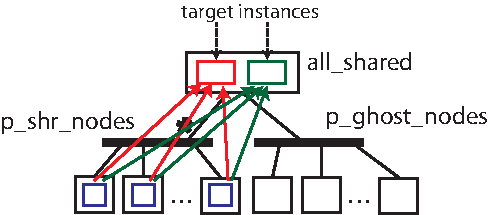
\includegraphics[scale=0.9]{figs/CloseOperation.pdf}
\caption{Example Close Operation from the Circuit Simulation\label{fig:exclose}}
\end{figure}

One important detail regarding the premapping
traversal is that it must always be performed
on the same node as the parent task before any
physical region tree meta-data is moved to
remote nodes for mapping (see 
Chapter~\ref{chapter:distributed} for more
details).  The reason for this is that we
need to be sure that close operations are
performed exactly once, as the updates that
they perform to the region tree meta-data
must be serializable. Therefore, since all
sub-tasks start on the same node as the 
parent task, by requiring them all to complete
the premapping traversal on the parent task
we can be sure that close operations are
only performed one time. Requiring premapping
traversals to be done on the parent node
also has the added benefit of reducing the 
amount of meta-data that must be sent to
other nodes for remote mapping as only 
the sub-trees of logical regions requested
by the region requirement are needed for
the remaining stages.

\subsection{Mapping Traversal}
\label{subsec:maptraversal}
The second traversal that is performed is
the {\em mapping traversal}.  The purpose
of this traversal is two-fold: first, in
the case of projection region requirements
it traverses from the region tree node  where
privileges were requested to the region tree
node where mapping will take place, and 
second, it actually selects which physical
instance to use (or re-use) for mapping the
region requirement without making it valid. 
Unlike the premapping traversal
that was required to be performed on the
origin node of the task, the mapping
traversal can be performed remotely. To
map remotely, the necessary meta-data for
the physical region tree must be moved
to the target node.  We discuss movement
of meta-data for remote mapping further
in Chapter~\ref{chapter:distributed}. We
now cover the two phases of the mapping
traversal in more detail.

The first phase of the mapping traversal
computes the path from where the original
region requirement requested privileges
to where the individual task's region
requirement is requesting privileges. For
individual tasks and other operations
that use normal region requirements, this
path consists of a single node and requires
no work.  However, for index space tasks
that can use projection region requirements
(see Section~\ref{subsec:indextasks}), this
path can be arbitrarily long. 
Figure~\ref{fig:mapaths} shows the difference
between the premapping and mapping paths for
a projection region requirement of the 
{\tt update\_voltages} task from the circuit
simulation. The premapping traversal to the
{\tt p\_shr\_nodes} partition is done exactly 
once for the index space task. However, the 
mapping traversal is done individually on 
a point-wise basis from the {\tt p\_shr\_nodes}
partition to the logical regions on which
each point task is requesting privileges.

\begin{figure}[t]
\centering
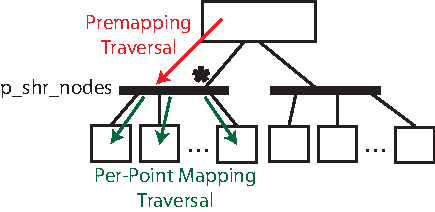
\includegraphics[scale=0.9]{figs/PremappingTraversal.pdf}
\caption{Premapping and Mapping Paths\label{fig:mapaths}}
\end{figure}

The one important invariant that is different in
the mapping traversal from the premapping
traversal is that no close operations will
need to be performed as part of the mapping
traversal.  By using projection region requirements
to scope an upper bound on the privileges
requested by all tasks in an index space
task launch, we guarantee that all the necessary
close operations are computed and performed
as part of the index space task's premapping,
and therefore no close operations need to
be performed for point tasks within the 
index space task. As part of the mapping
traversal, the necessary sub-trees within
the region tree physical state are opened
to reflect that there are potential users
in the sub-tress.

After arriving at the destination node, 
the traversal then attempts to either find or
create a physical instances of the target
logical region to hold the data necessary
for satisfying the region requirement.
Determining the physical instance to select
requires input from the mapper since both
the placement of the physical instance as
well as its layout can impact the performance
of the application. We therefore ask the
mapper to assign a ranking of memories and
set of properties (e.g. layout information)
for all region requirements prior to performing
any of the mapping traversal by invoking
the {\tt map\_task} mapper call. The mapper
decorates the region requirements for the
task with its chosen ranking of memories and
required set of constraints on the layout
of the physical instance. Based on these
requirements, the runtime then sequentially
walks through the list of memories, and for
each memory attempts to either find or 
create a physical instance that meets the
constraints. When looking for a physical
instance that meets the constraints, the
runtime can select any instance from the
current node, or from any of the nodes above
it.  In the process of selecting nodes
from further up in the tree, we must be careful 
to invalidate fields from higher nodes
when those same fields for instances lower
in the tree contain dirty data. It is safe
to re-use the instances, but it will require
additional data movement to bring the fields
up-to-date. If no instance can be found or 
created for any of the region requirements 
then the mapping stage fails, and the mapper
is notified with the {\tt notify\_failed\_mapping}
mapper call. 

It is important to note that after the mapping
traversal is complete, we do not actually
issue any data movement operations for
updating physical instances.  Instead this
is done in the third traversal when we register
the physical instances (see 
Section~\ref{subsec:regiontraversal}). The reason
for this discrepancy is that in some cases, we
may only discover that a mapping has failed
after we have completed the mapping traversal
for several other region requirements. In these
circumstance, we need to free any physical instances
that we have created as part of the mapping 
traversal in order to avoid resource deadlock.
Rolling back these allocations would be complicated
if we had already issued copy operations to bring
the instances up-to-date. Therefore, we defer 
issuing any of these operations until we know for
sure that the mapping will be successful for 
all region requirements that a task requested.

In some cases, the mapper for a task may determine
that it does not require the creation of a physical
instance for a region requirement, and instead
only needs to pass privileges for the task to
further sub-tasks. Under these circumstances we
allow mappers to request {\em virtual mappings}
of a region requirement, which will not create
a physical instance.  Virtual mappings trivially
succeed in the mapping traversal phase. We discuss
the implications of virtual mappings in more
detail in Section~\ref{subsec:virtualmap}.

\subsection{Region Traversal}
\label{subsec:regiontraversal}
Once we have completed the mapping traversal
for all region requirements for a task, we know
that the mapping stage of the pipeline will
be successful. At this point it is safe to 
issue the necessary copy operations for ensuring
that the physical instance selected for each
region requirement has the correct version of
the data for the requested fields of the logical region. 
To issue the necessary copies required for making
the physical instances valid copies of the data, 
we first determine the set of fields that are invalid. 
It is possible that the instance that we have selected
is already valid for all the fields at the target
logical region, in which case no copies need to be
issued. Its also possible that one or more fields
are invalid, and therefore must be updated.

To perform the updates we first compute the
set of {\em valid instances} for each field. The
valid instances are the instances that contain
valid data for the specific fields that 
need to be updated from the perspective of the
target logical region. When computing the set of
valid instances, it is legal in some cases to
use physical instances from logical regions
higher in the region tree. Determining when 
instances from logical regions higher in the
region tree can be used is non-trivial due to
the existence of buffered dirty data within
the physical instances. To compute the valid 
instances from the perspective of a logical
region $R$, we start at $R$ and traverse
back up the tree.  As we traverse up, we maintain
a field mask that describes the {\em search fields} for 
which we are looking for a valid instance. Before 
traversing up the next node, we remove any fields 
that contain dirty data at the current node from the 
search field mask, thereby preventing us from considering 
instances higher in the region tree as valid. At each
node we look for physical instances that contain
valid data for the target field.  We record all
physical instances that have valid data for any
of the fields for which we are searching.  We 
maintain a field mask for each of these physical
instances; the field mask records the subset of fields for
which they contain valid data.  When the search field
mask is empty, or we reach the region at the top
of the parent task's privilege context, we can
return the set of valid instances.

Figure~\ref{fig:validtrav} depicts an example search
for valid instances in a region tree for two fields
$A$ and $B$. Starting from the query region,
the traversal proceeds up the tree. Initially both
the $A$ and $B$ fields are in the search field mask. 
Instance $I_4$ contains a valid copy of $A$ and is
added to the result set. We then progress to the 
parent logical region where we discover instance
$I_3$ that contains a valid instance for both $A$
and $B$ which is added to our result set. Before
traversing the grandparent region, we first must
remove field $A$ from the search field mask because it
is a dirty field in the parent logical region. This
indicates that any instances in ancestor regions will
contain stale data for field $A$. Therefore, when we
arrive at the grandparent region, we can safely add
instance $I_2$ to the result set for field $B$. 
However, we cannot add either $I_1$ or $I_2$ for 
field $A$ because $A$ is no longer in our search
field mask. Ultimately, our result set indicates that
instances $I_3$ and $I_4$ contain valid data for
field $A$ and instances $I_2$ and $I_3$ contain
valid data for field $B$.

\begin{figure}[t]
\centering
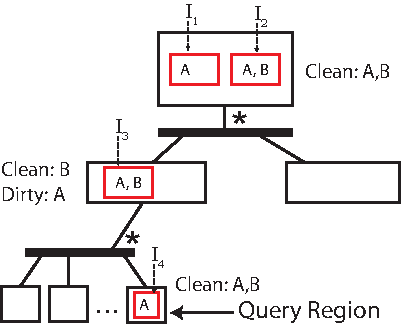
\includegraphics[scale=0.9]{figs/ValidViews.pdf}
\caption{Example Valid Instance Views Computation\label{fig:validtrav}}
\end{figure}

Once we have the valid set of instances for
all the fields we need to update, we can issue
the copy operations to update our target
instance. In many cases, there may be multiple
physical instances that can serve as source
instances for the copies. Since the choice
of sources may impact performance, we consult
the mapper when necessary about selecting the
sources for copy operations. If there are multiple
valid instances, we query the mapper
to rank the memories that should serve as 
sources for the copies. We invoke the mapper
by calling the {\tt rank\_copy\_sources} mapper
call and provide the mapper with a list of 
the memories that currently contain valid 
physical instances and the memory of the 
destination physical instance. The mapper
returns an ordered ranking of the memories
or a subset of the memories in which case
the other memories are appended to the ranking
in a random order to maintain correctness\footnote{
Even if the mapper does not rank all memories, the
runtime still needs to guarantee that copies get
issued to update all fields with valid data, hence 
the necessary appending to the list.}. Using this ranking, 
the runtime then issues the necessary update
copies from physical instances based on the
ranking of memories. Only one copy needs to
be issued for each field.  Where possible,
copies are issued jointly as gathers from
multiple physical instances over multiple
fields to afford the low-level runtime 
maximum visibility in optimizing copy 
routines and fusing together data movement
to ensure bulk data transfers.

Now that we have an up-to-date physical instance
at the target logical region, we lastly
need to flush any dirty data from below in 
the tree up to the current logical region.
We examine all of the open children to 
determine if they have any dirty data. If
they do we issue a close operation with 
our selected physical instance as the target.
This ensures that any dirty data below in
the tree is properly added to our physical
instance. The privileges requested by 
the region requirement determine if the
sub-trees can be left open: read-only privileges
permit sub-trees to remain open while read-write
and reduce privileges do not since these privileges
invalidate the instances in the
sub-trees. After any close operations
are performed we can register our new
physical instance as a valid physical
instance at the current node in the 
region tree.  If any dirty data was flushed
up from sub-tress, then we update the
set of dirty fields at the current node
and invalidate any other physical instances
at the current node (since they are no
longer valid).  We then add our physical
instance to the list of valid physical
instances for the fields requested by
our region requirement.

\subsection{Physical Instance Traversal}
\label{subsec:instancetraversal}
After we update all the field data for
each physical instance that is going to be
used for a task, we now need to
determine the set of dependences that 
must be satisfied before we can safely
use each physical instance. These dependences take
the form of low-level runtime events 
corresponding to other tasks and operations
that are already using the physical
instances. Once we have computed the set
of event preconditions, we can merge
them together into a single low-level
runtime event and launch the corresponding
low-level runtime task with the proper
event precondition.

To determine the event preconditions for
a new user, we perform a traversal over
the {\em instance view tree} for the target
physical instance. An instance view tree is a
data structure that mirrors a region tree and
tracks users of a physical instance from the
perspective of different logical regions. We
cover the details of instance view trees in
further detail in Section~\ref{subsec:instviews}.

Figure~\ref{fig:instrav} shows the instance views 
in the instance view tree that need to be checked 
when performing a physical instance traversal for a 
new user of a physical instance. Views highlighted 
in red must be visited to check for dependences, while 
those in blue can be skipped. Specifically, the 
user must visit the instance view at which it will be 
registered as well as all ancestor views and all
sub-tree views. While it is possible for there to 
exist interfering users from the blue instance views,
they will be detected in the ancestor parent views
because all users are registered in all their ancestor
instance views as well (see Section~\ref{subsec:instviews}
for more details). At each instance view that is
traversed, the user being registered examines all 
the currently registered users for interference
based on the same criteria as was presented in
Section~\ref{sec:noninterference}. To aid in 
discovering disjointness on logical regions
of users registered in ancestor instance views,
we also annotate users with which sub-tree they
came from, allowing region disjointness to be
determined without traversing any sub-trees.
The output of the instance view traversal is a
set of low-level runtime events that describe
all the interfering users in the instance view
tree. The runtime can then use this set of events
to construct a single low-level runtime event
that serves as the precondition for an operation
using the physical instance. Once the
analysis is complete, the user is itself registered
in the tree with its termination event. The user
is registered in all instance views from the view
in which it is requesting privileges up through all ancestor
instance views to the root of the instance view tree.

\begin{figure}[t]
\centering
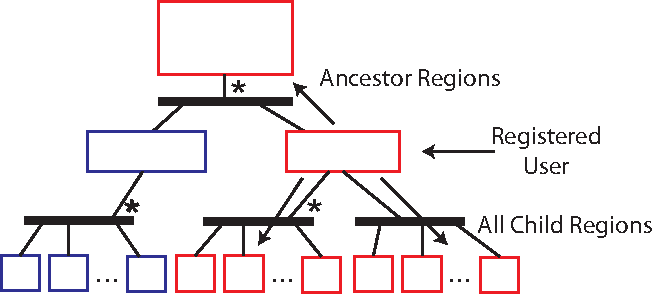
\includegraphics[scale=0.9]{figs/InstanceViewTraversal.pdf}
\caption{Instance View Tree Traversal\label{fig:instrav}}
\end{figure}

After we have completed the physical instance
traversal for each of the region requirements
of a task, we have the set of all low-level
runtime events that must trigger before the
task can run.  Using the low-level runtime 
interference, we merge all these events together
and launch the task with the computed event
as a precondition.  The event that is returned
is used as the event that marks when the task
will be done executing and we use it for registering
the user in the instance view tree.

One important detail is that the same instance
view tree traversal algorithm described here is
also used in Section~\ref{subsec:regiontraversal}
to compute the preconditions for issuing copy
operations to and from physical instances.  Both
the source and destination region trees are 
analyzed.  Copies take the form of a special
kind of user with exclusive coherence and 
either read-only, read-write, or reduce 
privileges depending on the kind of copy being 
performed. The low-level runtime also takes
an event precondition on copies and returns
an event for describing when the copy will
be finished. Using this low-level event,
copies also register themselves as
users in the instance view trees to ensure
correct dependence analysis when computing 
the set of precondition events for any
future user.


\section{Physical Region Tree Data Structures}
\label{sec:phystree}
Much like the state required for the logical
dependence analysis described in 
Chapter~\ref{chapter:logical}, our physical 
region tree traversal for performing the mapping
analysis also requires the storage of meta-data
on nodes in the region forest. While some of the
the meta-data stored on individual nodes is the
same as the logical meta-data, some aspects 
are different.  We describe the specific
state required for each node in 
Section~\ref{subsec:physstate}.
In addition to storing state on each node, the
physical region tree traversal will also require
two new kinds of data structures:
{\em instance managers} for tracking
physical instances and {\em instance views}
for tracking the operations that
are using the physical instances. 
We provide descriptions of these data
structures in Section~\ref{subsec:instmanagers}
and \ref{subsec:instviews} respectively.

Similar to the logical dependence analysis data,
physical region tree traversal meta-data is 
decorated on nodes of the region tree forest.
To differentiate the state for different
task executions, we again use the notion of
contexts, initially introduced in 
Section~\ref{subsec:logicalctx}. The same context
ID that is allocated for non-leaf parent tasks 
for performing dependence analysis is used for
performing the physical region tree traversal
for sub-tasks launched within a parent task
(with the exception for virtual mappings discussed in 
Section~\ref{subsec:virtualmap}). Each region tree
node maintains a separate array of physical meta-data
objects that can be directly indexed by the
context ID, allowing traversals from different
contexts to occur independently.

\subsection{Region Tree State}
\label{subsec:physstate}
On each node of the region tree, several different
meta-data structures are maintained. First, similar to
the logical state data, each physical state for a
node tracks which of the sub-trees are {\em open}.
There is a slight difference in the definition of open
for the physical state of the region trees: a sub-tree
is said to be open for a field $f$ if it contains at
least one valid physical instance for $f$ at some
node in the sub-tree. Note that this is different
from the logical state where a sub-tree was considered 
open if there were operations registered in the sub-tree.
Unlike the logical region tree state, where both
field and the privilege modes for open sub-trees
were tracked, the physical region tree traversal
only needs to track which field of sub-trees are
open.  The reason for this is that the logical 
region traversal memoized the results of the privilege
analysis when the close operations were recorded
for each operation.  By applying the close operations
as part of the premapping traversal discussed in 
Section~\ref{sec:premapping}, sub-trees will be
implicitly open with the proper privileges (e.g.
multiple sub-trees will only be open if multiple
read-only or reduction tasks are active in those
sub-trees). Open information for individual fields
are still required to know whether a sub-tree is
actually open or whether it was closed by another
task in the same epoch during its premapping
traversal.

The second piece of meta-data state stored on each 
region tree node is a field mask that tracks dirty
information. The dirty field mask records which
fields at the current region tree node contain
dirty information (e.g. have been written to).
When a region tree is going to be closed, dirty
information is necessary for computing which
data movement operations are required to propagate 
information back to higher levels in the region tree.

The final component of the physical state at
each region tree node is a list of {\em valid
instances}.  This list contains a list of 
instance view objects (see 
Section~\ref{subsec:instviews}) that represent
physical instances that contain a valid version
of data from the local region tree node. Each
valid instance is accompanied by a field mask
that describes the specific fields for which
the physical instance contains a valid instance
of the data.  It is often possible that a
physical instance only contains valid data for
a subset of the fields for which it has 
allocated space.

\subsection{Physical Instance Managers}
\label{subsec:instmanagers}
When physical instances are allocated, the
Legion runtime creates a {\em physical instance 
manager} to keep track of the properties of the 
physical instance. These properties include the 
memory in which the instance is allocated, the location 
in that memory, the layout of the fields, and the 
linearization of the index space.
When copies are issued either to or
from a physical instance, the physical instance
manager is responsible for generating the necessary
instructions for directing the low-level runtime
about how to perform the copy. For instances with
hundreds or thousands of fields, this information
can be expensive to compute.  We therefore cache
the meta-data required for issuing copies so that
it can be re-used when similar copies are requested.

Since instance managers are often large objects that
contain no context specific information, we deduplicate
them across physical contexts and ensure that at
most one physical manager exists for each physical
instance on a single node. We describe how physical
managers are lazily migrated between nodes in 
Chapter~\ref{chapter:distributed}.  The per-node 
uniqueness property guaranteed by physical instance
managers also serves a useful purpose in our 
garbage collection mechanism for physical instances 
that we describe in Chapter~\ref{chapter:garbage}.

\subsection{Physical Instance Views}
\label{subsec:instviews}
While instance managers are used to describe the
properties of a physical instance, we use a 
separate collection of objects to track the 
users of physical instances. An {\em instance view}
is an object that records all operations (e.g.
tasks, copies, inline mappings) that are 
using a specific physical instance from the
perspective of a specific logical region. A
physical instance initially created for a logical
region $R$ can serve as a valid physical instance
for any logical region in the sub-tree of $R$.
In some cases there might be multiple tasks using
the same physical instance from the perspective of
two disjoint logical sub-regions. In cases where
these tasks might be interfering on everything except
region disjointness, it is important to be
able to detect these cases to avoid false dependences.
By providing different instance view objects for
the same physical instance, we can maintain precise
information about how different users are using the
same physical instance and accurately detect when
dependences need to exist between users.

An instance view tracks the set of users of a 
specific physical instance from the perspective of
a single node in the region tree. The collection 
of instance view objects for a specific physical 
instance are therefore organized as a tree that 
mirrors the shape of the region tree from which 
the physical instance originates. For physical 
instances that contain valid data in multiple
contexts there is a separate set of instance 
views for each physical context within the region 
tree to ensure that users from different contexts 
do not need to perform non-interference tests 
against users from other contexts\footnote{
This is sound because of the hierarchical privilege
property: if two tasks are non-interfering then so
are any children they generate.}. All users are 
registered with instance views from the region 
in which they requested privileges to the 
root of the instance view tree. (Note
the root of the instance view tree is 
always the logical region that initially
created the physical instance.) Registering
users in this way will enable the simple
algorithm for finding interfering users
described in Section~\ref{subsec:instancetraversal}.
When a user is registered we record the privileges, 
coherence, and a field mask for describing which 
data is being accessed and how it is being accessed.
Each user also records a low-level runtime
event that will be triggered upon completion,
allowing later tasks to know when the user
is done using the physical instance.

As an important optimization for tracking the
users from the perspective of an instance view,
we also make use of {\em epoch lists}, similar
to the ones introduced in Section~\ref{subsec:epochlists}.
Epoch lists provide a mechanism for reducing the
number of users that must be tracked by each
instance view object. Identical to the epoch
lists of logical state objects, each instance view
object maintains two epoch lists: a current epoch
list and a previous epoch list. Whenever an added 
user dominates all of the previous users for a 
specific set of fields, we can remove the 
users of those fields in the previous epoch list
and filter the users from the current epoch list
into the previous epoch list. If the user does
not dominate the users in the current epoch list,
then it must also check for dependences in the 
previous epoch list and then add itself to the
current epoch list. The same observable condition
on domination applies: a user performing interference
tests must observe at least one other user of 
a field before being able to safely conclude that
it dominates that field.

Due to the large number of users that can 
accumulate in the current and previous epoch
lists, the runtime supports an important optimization
for reducing the number of users. By default,
lists are only modified by the standard instance view
traversal protocol described in 
Section~\ref{subsec:instancetraversal}. However, users
can also set an upper bound for the number of entries
in the epoch lists. Whenever the upper bound is reached,
the runtime performs three operations to compact the
epoch lists: user deduplication, privilege merging,
and field merging. The first compaction pass looks
for users from the same operation that have been 
fragmented on fields, due to epochs changing for different
fields at different times, resulting in multiple
versions of a user ending up in the previous epoch list.
The second compaction pass looks for users from the
same epoch on the same fields, and merges these users
together into a single user entry. Merging users also
requires generating a new event that represents all
the previous user events which is then stored in the
entry for the user.  Both of the first two compaction
passes still maintain the precision of the 
analysis.  The third operation reduces the precision
of the analysis and therefore may be optionally disabled
with the understanding that it will cause the upper
bound on the epoch lists sizes to be a soft upper
bound that may be exceeded.  In the third
compaction pass, users of different fields with the
same privileges are merged, again resulting in a single
merged event to represent multiple users. The resulting
users must contain a union of all the fields that 
were merged, potentially resulting in false dependences
being created between operations, but at the benefit
of a hard upper bound on epoch list sizes.

\section{Special Cases}
\label{sec:physicalcases}
Unlike the dependence analysis stage of the pipeline
that maintains a relatively homogeneous implementation
independent of the privileges and coherence of
region requirements, many of the special features of 
the Legion runtime must be handled differently in the 
mapping stage of the operation pipeline.
The reason for this is simple: the mapping stage 
is where the logical description of Legion programs
is targeted at a specific target architecture. It is 
therefore this stage that must handle the cross-product 
of interacting Legion features and how they are mapped
onto the hardware.  We discuss the implementation of
several of the more important features in this section.

\subsection{Supporting Reduction Instances}
\label{subsec:physreductions}
One of the important features of the Legion programming
model is that reduction privileges permit tasks to 
be non-interfering. In order to support this feature, 
Legion takes advantage of specialized {\em reduction
instances} provided by the low-level runtime \cite{Realm14}.
Reduction instances are a special kind of physical 
instance that only support reduction operations; 
arbitrary reads and writes are not permitted. The low-level
runtime provides two kinds of reduction instances:
reduction-list instances and reduction-fold instances.
Reduction-list instances buffer reductions as a
list, while reduction-fold instances maintain
separate entries for each row in an index space, but
at the significantly smaller cost of only needing
to store the {\em ride-hand-side} (RHS) value
of the reduction operator, which is commonly smaller
than the target field of the reduction. If multiple
reductions are applied to the same row, a
reduction-fold instance can perform a {\em fold operation}
to reduce the two intermediate values together, thereby
reducing the amount of information that must be stored
in the reduction instance\footnote{A fold operation 
has the type $RHS \rightarrow RHS \rightarrow RHS$, reducing
two elements of the $RHS$ type to one. Fold operations 
are required to be associative and commutative.}.
Reduction-list instances work better for tasks 
that are performing sparse reductions, while reduction-fold
instances work best for tasks performing dense reductions
(and when a specialized fold operator is not defined for
the reduction). Since the choice of reduction instance
can have an impact on performance, the decision of the
type of reduction instance to use is made by the
mapper as part of the {\tt map\_task} mapper call.

For all region requirements that request reduction
privileges, the runtime currently requires that a 
reduction instance be made. This restriction is what
permits tasks requesting reduction-only privileges
on otherwise interfering regions to both map and
execute in parallel. To track reduction instances,
each of the physical state objects for tracking
physical traversal meta-data (described in 
Section~\ref{subsec:physstate}), is updated to
track all the fields that currently have outstanding
reductions, as well as a collection of reduction
instances available for the current region tree node.
When close operations are performed, reductions are
always flushed back up to the target physical instance
after all other dirty data has been copied back. This
implementation stems from a very important invariant
maintained by the logical region tree dependence
analysis: whenever sub-trees are open in reduction mode,
there can never be any dirty data below the reduction 
operations. If dirty data does exist in a sub-tree before
a reduction is mapped, a close operation  is always performed
before the tree is opened for reduction operations.
This invariant significantly simplifies the reasoning 
about reductions and allows all reduction operations
to be performed last as part of close operations. We
will leverage this invariant again in Section~\ref{subsec:composite}
when we discuss composite instances.

\subsection{Post Task Execution}
\label{subsec:postexec}
One important aspect of task execution in Legion is
that after a task has finished executing, the data
associated with the logical regions on which the task
held privileges may actually be strewn across the 
machine in many physical instances created by sub-tasks
and other operations launched by the task.  However,
the sibling tasks of the parent task have made mapping
decisions contingent upon the output of the task being
stored in the physical instances that the task initially
mapped. Therefore, after a task has finished launching
sub-tasks, the Legion runtime issues close operations on
the fields of any region trees on which a task held
either read-write or reduction privileges. The result
of applying these close operations is that any dirty 
data residing in other physical instances throughout
the memory hierarchy is flushed back to the physical
instance that the task initially mapped. Since the
purpose of these close operations is purely to 
aggregate dirty data, there is no need to issue
close operations for region requirements with 
read-only privileges, as it is impossible for any
dirty data to reside in these region trees. Issuing
of close operations for region trees with potentially
dirty data is necessary for correctness of Legion
applications.  However, as we will see in 
Section~\ref{subsec:virtualmap}, there are some
mapping decisions that can be made that eliminate
the need for the close operations.

\subsection{Handling Virtual Mappings}
\label{subsec:virtualmap}
The hierarchical nature of the Legion programming model
encourages tasks that recursively launch sub-tasks.
The Legion programming model also requires that privileges
for regions be passed from parent tasks down to sub-tasks.
For many intermediate tasks in the task tree, it is
unnecessary to instantiate a physical instance for
the region requirements requested by the task.  In some
other cases the logical regions may be too large to fit 
in any memory in the machine.  Under these circumstances,
it is useful for a mapper to be able to request that 
a region requirement be {\em virtually mapped}. In a
virtual mapping, no physical instance is actually created
for the region requirement, but the task is still granted
the requested privileges and can pass them down to any 
sub-tasks that it launches.

When a virtual mapping is performed for a task, there no
longer exists a canonical physical instance of the data
when the task starts.  Any sub-tasks or other operations
that request privileges on the regions therefore need to be
mapped differently to ensure that they observe the correct
versions of the data. Instead of mapping within the context
of the parent task (which is meaningless because of the
virtual mapping), we instead map these operations within
the context of the closest enclosing ancestor task that 
did not virtually map the region, or the ancestor task
that created the logical region. It is important to note
that this definition is inductive, and allows for multiple
nested tasks to all perform virtual mappings, which is
important for writing scalable Legion applications with
many layers of nested tasks.

Since all sub-tasks and other operations that acquire
their privileges from a virtually mapped region are not 
mapped directly in the parent task context, but instead 
are mapped in an ancestor task context, there is no need
to explicitly issue close operations on the region trees
after the task has completed. Instead the information
about where data is located has already explicitly flowed
back into the ancestor task context. To be sound, this
process requires a slight modification to the handling
of mapping dependences discussed in 
Section~\ref{sec:mapdepgraph}. Tasks that request
virtual mappings on at least one region requirement
cannot be considered mapped until they have finished executing
and any sub-tasks or other operations that they launched
have also finished mapping. This guarantees that all the
necessary mapping information has flowed back into the
ancestor task's context before any sibling tasks of the
parent task with mapping dependences on the parent task 
can begin to map. Virtual mappings therefore present an 
interesting trade-off opportunity for mappers: using 
non-virtual mappings can enable more parallel mapping 
opportunities, at the cost of creating intermediate physical 
instances, while virtual mappings negate the need for 
creating intermediate physical instances while serializing 
the mapping process. Determining whether to use virtual 
mappings is therefore a performance decision that is always
left to be determined by the mapper for a task.

Importantly, the same machinery that is used to handle virtual 
mappings is also used for handling logical regions that are 
created and returned from a task. Effectively, a newly
created logical region is one that was anonymous and virtually
mapped before the task was executed.  If the newly created
region is not deleted before a task completes execution,
the privileges associated with that region flow back to
the enclosing parent task. To be correct, the corresponding
state of the newly created region must also flow back to
the enclosing parent task context. The Legion runtime handles
this by always performing physical region tree analyses for
newly created regions in the context of the earliest ancestor
of the creating task on the local node. By using this context,
the necessary meta-data does not have to be copied back to 
enclosing task contexts as privilege information propagates
back up the task tree, and instead only needs to be copied
when moving across nodes, under which circumstances it would
need to be moved anyway.  We discuss the movement of physical
state data in detail in Chapter~\ref{chapter:distributed}.

\subsection{Optimizing Virtual Mappings with Inner Tasks}
\label{subsec:innertasks}
Virtual mappings have the detrimental effect of increasing
the length of critical paths in the mapping process because
sibling tasks of a parent task $P$ with virtual mapped
regions must wait for all child operations of $P$ to map. In the
general case this requires waiting for $P$ to execute in
order to discover all the children. However, because of 
deferred execution, it may be a significant amount of time
before $P$ actually begins, thereby delaying the mapping of
any siblings of $P$. To reduce this latency, Legion permits
an important optimization called the {\em inner task}
optimization to reduce the latency of the mapping process
when virtual mappings are used.

An inner task is a Legion task that only requests 
privileges on logical regions and never actually inspects
the data contained in the logical regions\footnote{The
term {\em inner task} originated in the Sequoia programming
language where inner tasks were only permitted to launch
sub-tasks with {\tt mappar}, {\tt mapseq}, or {\tt mapreduce}
operations and could have no control flow dependent on 
array data. The Legion definition of inner tasks is more
flexible and permits arbitrary code execution, but with the
same restriction that logical region data cannot be accessed.}.
Since the parent task $P$ guarantees that it will not be
accessing any data within its logical regions as part of its
execution, the Legion runtime can actually start the execution
of $P$ immediately. Any child tasks of $P$ will automatically
pick up the correct dependences by traversing in the context
of $P$'s parent task. The inner task optimization also works
if $P$ had any non-virtually mapped regions: non-inner task
children of $P$ simply add the original precondition events 
for each physical region of $P$ that they depend on to 
their preconditions. Ultimately, the inner task optimization
reduces the latency of the mapping process by permitting
the runtime to execute $P$ early, which leads to early 
discovery and mapping of children of $P$.


\subsection{Deferring Close Operations with Composite Instances}
\label{subsec:composite}
In early versions of the Legion runtime, all close
operations on a physical region tree required the mapper 
object to select one or more physical instances from the
region tree node at the root of the sub-tree being 
closed to serve as the target of the close operation.
This requirement, while unobtrusive in most cases, still
results in some cases for which it is impractical. For example,
if the region node at the root of the sub-tree being closed
constitutes a very large logical region that cannot fit in
any memories in the machine, then the close operation cannot
be performed. Furthermore, in some cases, building an instance
as the target of a close, and then opening a new sub-tree
results in a many-to-one followed by one-to-many communication
pattern that serializes data movement through a single memory
in the machine. Under some circumstances it is better to 
encourage many-to-many communication patterns.  To address 
these issues, Legion maintains support for 
{\em composite instances}.

A composite instance is a snapshot of the physical state
of a specific sub-tree in the region forest for one or 
more fields. Every composite instance supports multiple
views onto it from other nodes in the region tree forest.
These {\em composite views} share the same interface as
instance view objects (see Section~\ref{subsec:instviews}),
but instead of being backed by a specific physical instance,
are instead backed by a collection of physical instances
from the captured region tree state.

Composite instances can never be used directly by tasks
or as the target of copies.  Instead, they can only
serve as the source for copy operations.  When a copy
is issued from a particular composite view of a composite
instance, all of the potentially overlapping parts of the 
captured tree state must be explored to determine the
actual copies that must be performed. In essence, this
analysis is an intersection test: for some target region 
$R$ in one sub-tree, find all of the regions in another 
sub-tree that potentially intersect with $R$ and issue
copies from physical instances in those regions to the
target physical instance to ensure that the physical
instance of $R$ contains valid data. 

Issuing copies from composite instances can be expensive,
therefore our implementation attempts to minimize any
overhead. First, for each field, every composite view 
maintains a pointer to the node in the captured sub-tree
that dominates the logical region being represented by
the composite view.  Since these nodes are often well below 
the root of the composite instance, this reduces the number
of nodes that must be considered for intersections
when issuing copies. To further reduce overhead, the runtime 
also memoizes the results of domination and intersection tests 
between different index spaces and index partitions, allowing
the cost of these tests to be amortized across the creation
of many composite instances (with the exception that domination
tests must be invalidated under dynamic allocation similar
to completeness tests, see Section~\ref{subsec:logicalshape}).

The impact of composite instances is profound. Instead of
having to rebuild a physical instance at the root of a
sub-tree in a memory, instead a composite instance is
built.  When other sub-trees are opened, the necessary
copies, and only the necessary copies, are issued to
bring physical instances in the new sub-tree up to
date.  Most importantly, multiple tasks that open
a new sub-tree can be mapped in parallel, possibly
on different nodes, and composite instances permit
the necessary copies for updating each of the new
physical instances in parallel, increasing the amount
of data movement parallelism that is exposed to the
low-level runtime. Ultimately, composite instances 
allow applications to fully leverage the multiple
views onto logical regions enabled by the Legion
programming model's multiple partitioning feature
(discussed in Section~\ref{subsec:multiple}).
Supporting multiple partitions is essential for
modern supercomputing applications that go through
many phases of computation; composite instances
make the Legion implementation of multiple
partitions efficient.


\section{Parallelizing Physical Tree Traversal}
\label{sec:paratraversal}
Unlike the dependence analysis stage discussed in 
Chapter~\ref{chapter:logical}, it is possible for 
multiple non-interfering tasks within the same context 
to map in parallel on the same region tree.
We therefore need an approach to synchronize access
to the physical state data structures in the 
region tree forest. Before beginning our discussion
of our approach, we note that it is also possible
for multiple non-interfering sub-tasks within the
same context to be mapping in parallel on distinct
nodes; we discuss the management of distributed 
physical state across multiple nodes in detail in
Chapter~\ref{chapter:distributed}. In this section we 
focus on the synchronization necessary for performing
simultaneous mapping of non-interfering tasks in
the same context on a single node.

\subsection{Exploiting Field Parallelism on Premapping Traversals}
\label{subsec:parpremap}
The first synchronization guarantee that needs to be
upheld by the runtime involves the serializability of
mapping operations for individual fields. As we
discussed in Section~\ref{sec:premapping}, premapping
traversal of a field need to be serialized to ensure
that close operations are not duplicated. To maintain 
this property the context of the parent task
tracks which of the region trees have active
tasks performing premapping traversals. The parent
task only permits one premapping traversal to be 
active in a sub-tree for a given field at a time.
Note that this requirement only applies to premapping
traversal, allowing any arbitrary number of mapping
traversals to be occurring in parallel with any premappings
on a field; if they could not be performed in parallel, 
they would have been determined to be interfering in the 
dependence analysis stage. Additionally, because the
parent context tracks premapping traversals at the
granularity of fields, multiple premapping operations
on disjoint sets of fields may be proceeding in parallel.
This approach to premapping maintains the necessary
serializability guarantee while still permitting many
parallel traversal operations.

\subsection{Region Tree Locking Scheme}
\label{subsec:treelocking}
The second invariant that must be maintained is that
access to the physical state on every region tree 
node is serialized. The reason this is necessary is
that often many premapping and mapping traversals
might traverse the same region tree node in 
parallel. These traversal are clearly non-interfering,
but they still need to serialize their access to
common data structures in the physical state such
as the list of valid physical instances, which they
might both be mutating (in a non-interfering way)
at the same time.

To serialize access to the physical state object
in each region tree node, we create a low-level
runtime reservation object for the physical state
in each context. Low-level reservations provide
an atomicity primitive necessary for serializing
access to the physical state\footnote{Reservations
also allow us to encode that some operations are
read-only and are therefore not exclusive, while 
others operations require exclusive access for
mutating the physical state object.}. One important
property of the premapping and mapping
traversals is that if they are occurring in parallel
we already know that they are non-interfering.
This allows us to perform an important optimization
when accessing the physical state
object. Unlike traditional synchronization schemes
(usually based on locks), that require an entire
mutation of the state of an object to be done
atomically, traversals in Legion can take a
reservation to access the physical state, make
a thread-local read-only copy, and then release the
reservation. This local copy can then be safely
used for performing operations without holding
the lock. The reason that this is sound is that
the dependence analysis already guarantees that no
interfering traversal can be occurring in parallel,
so any updates made to the physical state while
a traversal is not holding a reservation are 
not important for correctness. By not requiring
traversals to hold state locks throughout the
duration of a traversal (either premapping or
mapping), a much finer-grained serialization
scheme is achieved which enables more parallelism
in the dependence analysis stage of the pipeline.

\subsection{Instance View Locking Scheme}
\label{subsec:viewlocking}
The final serialization guarantee that we must make
involves parallel traversal of the instance view
objects. Similar to the need to serialize access
to the physical state of region tree nodes in a
context, we also must serialize access to the 
data structures inside of physical instance view
objects. We again employ low-level runtime 
reservations as our atomicity primitives. The
non-interfering property of traversals guaranteed
by dependence analysis also applies to instance
view traversals (see 
Section~\ref{subsec:instancetraversal}). Therefore
we can employ the same optimization introduced in
Section~\ref{subsec:treelocking} of not needing
to hold a reservation for an entire mutation of 
an instance view. Instead it is common for traversals 
to acquire the reservations in read-only mode to 
search for interfering users, release the reservation, 
and then re-acquire it in exclusive mode to add a
new user to the epoch lists. 
Ultimately the two-phased locking (non-exclusive
followed by exclusive) allows more traversals
of instance views to occur in parallel.

